\documentclass{article}
\usepackage{url}
\usepackage[utf8]{inputenc}
\usepackage[pdftex]{hyperref}
\usepackage[margin=1in]{geometry}
\usepackage{amssymb}
\usepackage{amsmath}
\usepackage{braket}
\usepackage{graphicx}
\usepackage{verbatim}
\usepackage{hyperref}
\usepackage{multirow}
\usepackage{mathtools}
\DeclarePairedDelimiter{\ceil}{\lceil}{\rceil}
\hypersetup{
    colorlinks=true,
    linkcolor=blue,
    filecolor=magenta,      
    urlcolor=blue,
    citecolor=black,
}

\newcommand{\stamp}{\vcenter{\hbox{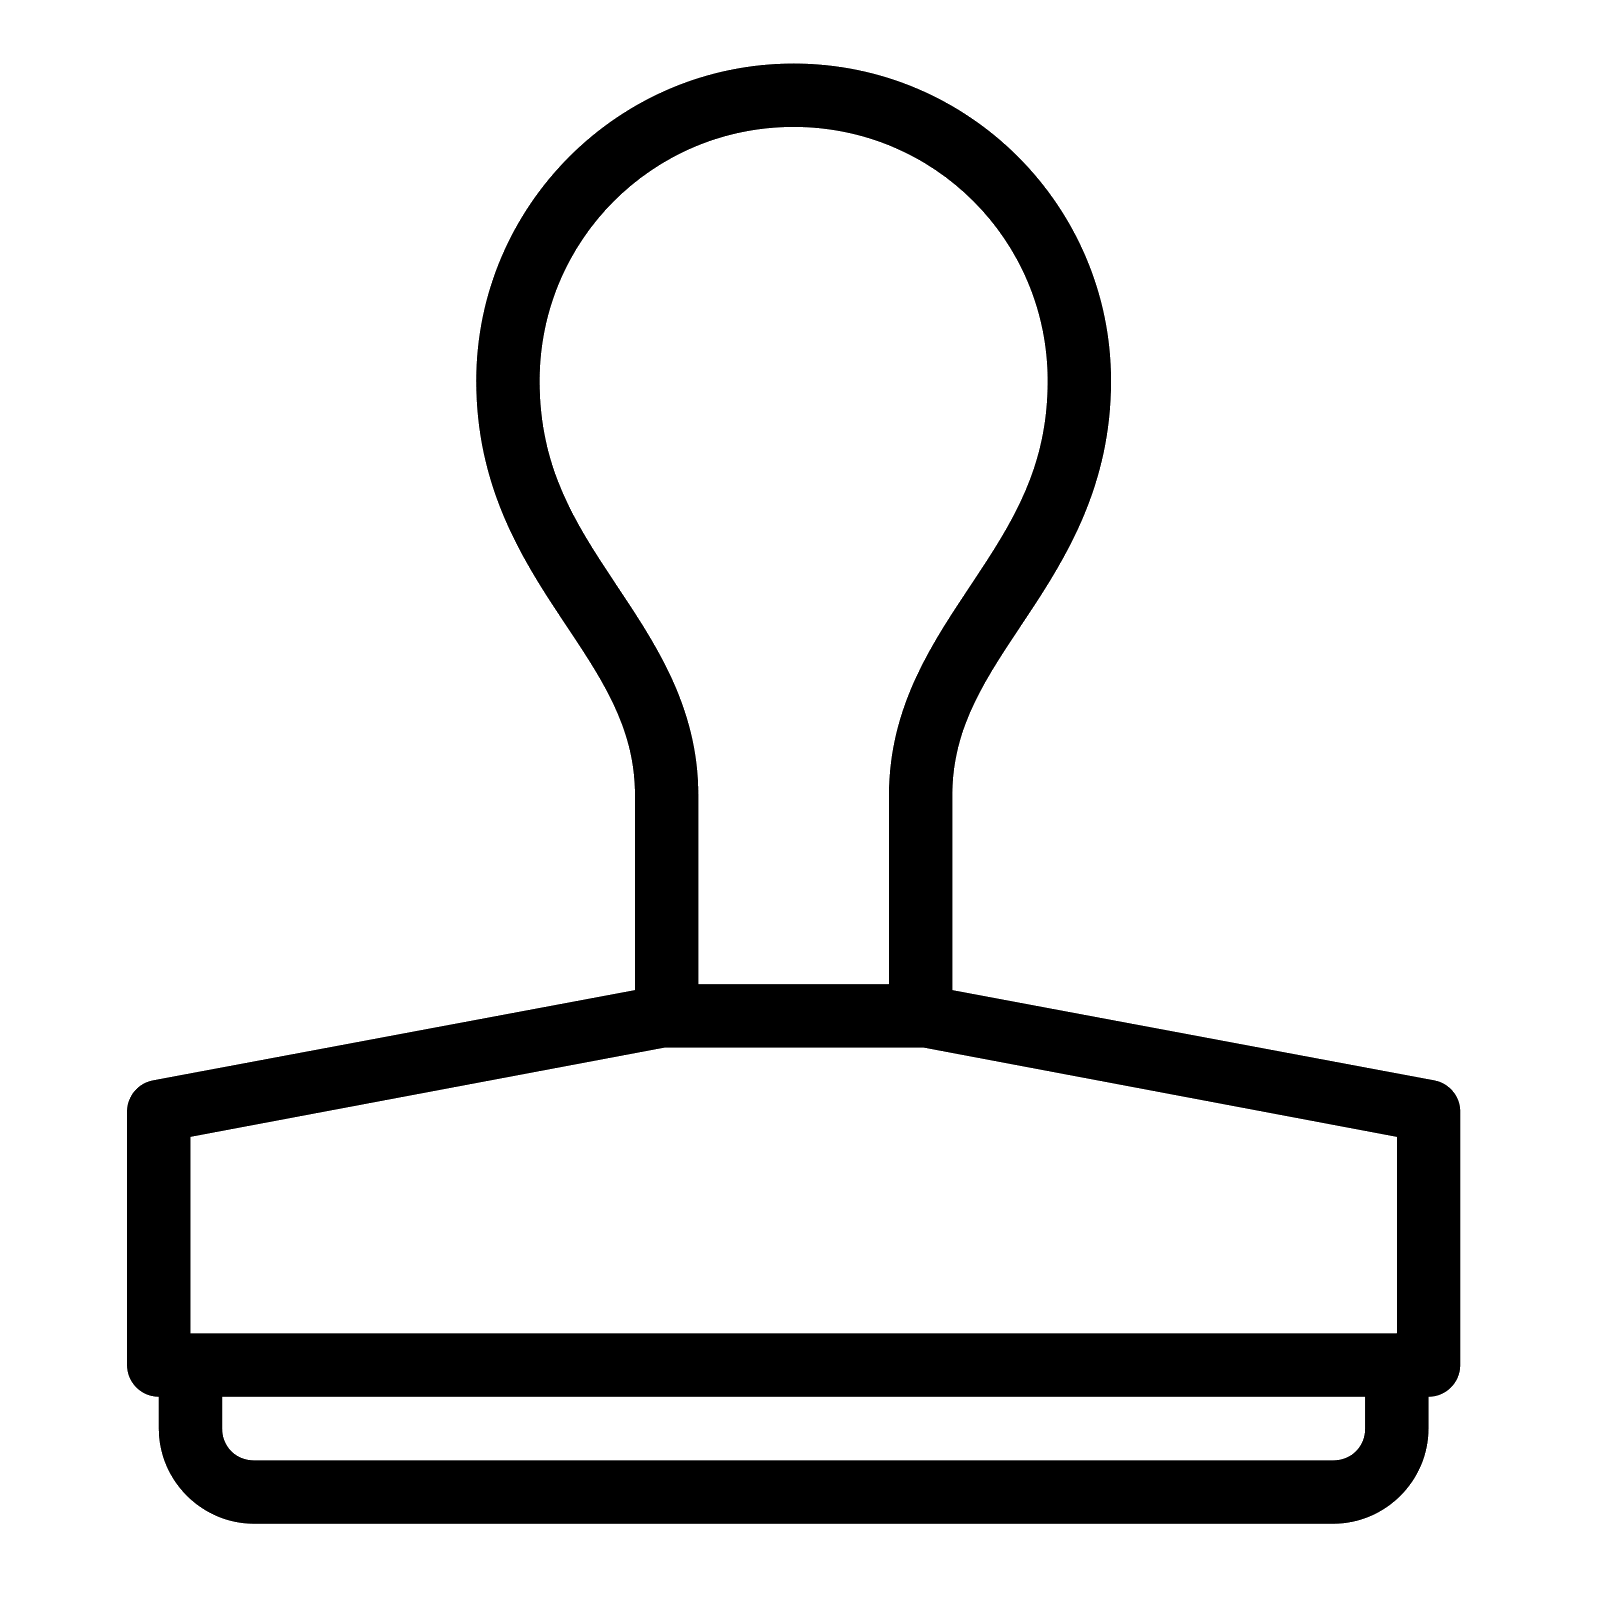
\includegraphics[height=1em]{rubberstamp}}}}

\begin{document}

\section{Definitions}
\textbf{\textit{Non-collapsing hash function.}} A hash function that is collision-resistant and not infinitely-often collapsing. (See \cite{zha17} for definitions of `collision-resistant' and `infinitely-often collapsing'. We can assume that there are adversaries who win the collapsing game for such functions with probability near 1. See \cite{gyz}, \cite{zha17} for examples of how one can boost the success probability of any bad adversary who breaks infinitely-often collapsing security so that it becomes a very good adversary.) \\

\noindent \textbf{\textit{Part-probabilistic non-collapsing hash function.}} A function $F(k, x, r)$ whose output takes the form $H(k, x) \: || \: R( H(k, x), r)$, where $H$ is a (deterministic) collision-resistant hash function, and $R$ is another function whose output is permitted to depend upon the randomness $r$ and the output of $H$. We require the following security properties of $F$:

\begin{enumerate}
    \item Collision resistance for $H$: For any quantum polynomial time adversary $A$,
    \begin{center}
        Pr[$H(k, x_0) = H(k, x_1) \wedge x_0 \neq x_1 \: : \: (x_0, x_1) \leftarrow A(k), k \leftarrow \{0, 1\}^\lambda$] $< \textsf{negl}(\lambda)$
    \end{center}
    \item (Infinitely-often) non-collapsing: There exists an adversary $A$ (consisting of two phases, $A_0$ and $A_1$) who can win the following game with probability $1-\gamma$, where $\gamma$ is negligible.
    \begin{itemize}
        \item The challenger has an input bit $b$.
        \item The challenger chooses a random key $k$, which it gives to $A_0$.
        \item $A_0$ creates a superposition $\ket{\psi} = \sum_x \alpha_x \ket{x}$ and submits this state to the challenger.
        \item The challenger generates a random $r$. It evaluates $F(k, \cdot, r)$ in superposition on $\ket{\psi}$, to get the state $\sum_x \alpha_x \ket{x, H(k, x), R(H(k, x), r)}$.
        \item The challenger does one of the following:
        \begin{itemize}
            \item If $b = 0$, it measures the last two registers, and returns the state $\sum_{x : H(k, x) = y} \alpha_x \ket{x, y, R(y, r)}$ to $A$.
            \item If $b = 1$, it measures the entire state, and returns the state $\ket{x_0, y, R(y, r)}$ (for some $x_0$) to $A$.
        \end{itemize}
        \item $A_1$ outputs a guess for $b$. If $A_1$ is correct, $A$ wins the game.
    \end{itemize}
\end{enumerate}

Note that, under this definition of `non-collapsing' (which mimics \cite{zha17}'s definition), the distinguisher $A_1$ is only guaranteed to exist \textit{if the challenger behaves honestly}. $A_1$'s success may depend upon $r$ being honestly generated, and upon $R$ being honestly run; it has no way of verifying that either is the case. In the generic hash function setting, we cannot guarantee that $R$ will be run honestly on a random $r$, and we cannot guarantee that the distinguisher $A_1$ which wins the game above will still be useful if this is not the case.

It is evident that the (deterministic) non-collapsing hash function is a special case of the part-probabilistic non-collapsing hash function, so that any NCH function is also a PP-NCH function.\\

\noindent \textbf{\textit{Chosen-y-secure hash function.}} A hash function $H(k, x)$ for which no quantum polynomial time adversary can win the following game with more than negligible probability:
\begin{itemize}
    \item The challenger chooses a random key $k$, which it gives to $A$.
    \item The challenger creates a uniform superposition over all inputs $x$ in the input space of $H$, and evaluates $H(k, \cdot)$ upon this superposition to obtain the state $\sum_x \alpha_x \ket{x, H(k, x)}$. It then measures the output register to obtain a state $\ket{\psi_y} = \sum_{x : H(k, x) = y} \alpha_x \ket{x, y}$ for some random $y$.
    \item The challenger gives $\ket{\psi_y}$ to the adversary. The adversary wins the game if it can recover $x_0, x_1$ such that $H(k, x_0) = H(k, x_1) = y$.
\end{itemize}

The collapsing security game can be defined in the same way for CYS hash functions that it is for collision-resistant hash functions.

Note that it is easy to construct a collision-resistance adversary from a chosen-$y$ adversary, and that, therefore, any collision-resistant hash function is also a chosen-$y$-secure hash function. This notion of `chosen $y$' security is close to that of second preimage resistance security; the former can be considered a strengthening of the latter to suit the quantum setting.

Note, in addition, that any PP-NCH function can be transformed into a CYS-NCH function. Chosen-$y$ security follows directly from the assumption of collision resistance for the deterministic part of the PP-NCH function. The non-collapsing property, meanwhile, follows from the fact that the chosen-$y$ setting already demands that $y$ is chosen randomly (presumably by some trusted party) if the CYS function's preimage security is to hold. Any construction using a chosen-$y$ hash function for its preimage security properties, therefore, must generate honest randomness when it generates $y$; and, as such, $y$ can be used as a source of randomness for the randomised part of the PP-NCH function.


\section{NCH implies BZ-GYZ}

\textbf{Claim.} Any non-collapsing hash function can be used to build a one-time signature scheme that is Boneh-Zhandry secure but not Garg-Yuen-Zhandry secure. \\

\noindent \textit{Scheme.} Given a non-collapsing hash function $F$, and an arbitrary BZ-secure one-time signature scheme $\mathsf{(Gen_{BZ}, Sign_{BZ}, Ver_{BZ})}$ (these are easy to produce; for example, the standard Lamport construction of a one-time signature scheme from a collision-resistant hash function is BZ-secure, according to \cite{BZ13b}), we construct a BZ-GYZ scheme $\mathsf{(Gen, Sign, Ver)}$ as follows.

\begin{itemize}
    \item \textsf{Gen} simply runs $\mathsf{Gen_{BZ}}$ to generate a pair of keys $\mathsf{(pk, sk)}$ for the BZ signature scheme.
    \item $\mathsf{Sign(sk}, m\mathsf{)} = F(m) \: \Vert \: \mathsf{Sign_{BZ}(sk}, F(m)\mathsf{)} = \sigma$. In other words, \textsf{Sign} applies the non-collapsing hash function $F$ to the message, signs the hashed message using the BZ scheme, and outputs the hashed message concatenated with the signature it obtains from the BZ signing oracle.
    \item $\mathsf{Ver(pk}, m, \sigma \mathsf{)}$ firstly hashes the message $m$ to obtain $F(m)$, and then verifies $F(m)$ using $\mathsf{Ver_{BZ}}$ and $\mathsf{pk}$.
\end{itemize}

\noindent \textit{Proof.} We firstly prove that this scheme is BZ-secure, assuming that $\mathsf{(Gen_{BZ}, Sign_{BZ}, Ver_{BZ})}$ is BZ-secure.

Suppose we have some adversary $A$ who is able to break the BZ-security of $\mathsf{(Gen, Sign, Ver)}$. The adversary $B$ can then use $A$ to break the BZ-security of $\mathsf{(Gen_{BZ}, Sign_{BZ}, Ver_{BZ})}$ as follows:

\begin{itemize}
    \item $B$ receives \textsf{pk} from its challenger. It passes \textsf{pk} on to $A$.
    \item $A$ creates a superposition of messages $\sum_m \alpha_m | m \rangle$ and gives it to $B$ as a query. $B$ computes $F$ on it in superposition, and then passes $\sum_m \alpha_m | m, F(m) \rangle$ on to its challenger, who computes $\mathsf{Sign_{BZ}}$ on it and returns the state $\sum_m \alpha_m | \: m, F(m), \mathsf{Sign_{BZ}(sk}, F(m)) \: \rangle$ to $B$. $B$ gives this state to $A$.
    \item $A$ outputs its (classical) forgery for $\mathsf{(Gen, Sign, Ver)}$. This forgery will take the form \\ $((m_0, F(m_0), \sigma_0), (m_1, F(m_1), \sigma_1))$, where $m_0$ and $m_1$ are two distinct messages.
    \item If $F(m_0) = F(m_1)$, then we have found a collision for $F$, which ought to be impossible, because we assume that $F$, a non-collapsing hash function, is collision-resistant. If $F(m_0) \neq F(m_1)$, then $B$ outputs $((F(m_0), \sigma_0), (F(m_1), \sigma_1))$ as its forgery for the $\mathsf{(Gen_{BZ}, Sign_{BZ}, Ver_{BZ})}$ scheme.
    \item If $A$'s success probability is non-negligible, then so is $B$'s.
\end{itemize}

Therefore, $\mathsf{(Gen, Sign, Ver)}$ is BZ-secure if $\mathsf{(Gen_{BZ}, Sign_{BZ}, Ver_{BZ})}$ is BZ-secure. \\

We now prove that the proposed scheme is not GYZ-secure. To do this, we use the fact that $F$ is non-collapsing. Let $D$ be an adversary which can break collapsing security for $F$. Following the proof to Theorem 13 in \cite{gyz}, we construct an adversary $A$ who uses $D$ to break the GYZ-security of $\mathsf{(Gen, Sign, Ver)}$. $A$ acts as follows:

\begin{itemize}
    \item $A$ queries $D$ to get a superposition of `messages' (preimages) $\rho = \sum_{m, m'} \alpha_m \alpha_{m'}^* | m \rangle \langle m' |$, and places this superposition $\rho$ in its message register. $A$ then flips a coin with outputs in $\{0,1\}$ and measures the message register iff the coin gives 0. This results in the following state:
    \begin{align}
        \frac{1}{2} \bigg[ \: |0\rangle \langle 0| \otimes \sum_m |\alpha_m|^2 |m \rangle \langle m| + |1\rangle \langle 1| \otimes \rho \: \bigg]
    \end{align}
    \item $A$ sends this state to the GYZ signing oracle, which signs it and places the signature in a newly created pair of signature registers. The result is then
    \begin{align}
        \begin{split}
        \begin{array}{c c c @{\:\:\otimes\:\:} c @{\:\:\otimes\:\:} c @{\:\:\otimes\:\:} c c}
            \frac{1}{2} \bigg[ & \sum_m |\alpha_m|^2 & |0\rangle \langle 0| & |m \rangle \langle m| &  |F(m) \rangle \langle F(m)| & \Ket{ \: \mathsf{Sign_{BZ}(sk}, F(m)) \: } \Bra{ \: \mathsf{Sign_{BZ}(sk}, F(m)) \: } & \\
            & + \sum_{m, m'} \alpha_m \alpha_{m'}^* & |1\rangle \langle 1| & |m \rangle \langle m'| & | F(m) \rangle \langle F(m')| & \Ket{ \: \mathsf{Sign_{BZ}(sk}, F(m)) \: } \Bra{ \: \mathsf{Sign_{BZ}(sk}, F(m')) \: } & \bigg]
        \end{array}
        \end{split}
    \end{align}
    $A$ measures the `$F(m)$' register (the third register from the left), to obtain the state
    \begin{align}
        \begin{split}
        \begin{array}{c c c @{\:\:\otimes\:\:} c @{\:\:\otimes\:\:} c @{\:\:\otimes\:\:} c c}
            \frac{1}{2} \sum_y \beta_y \bigg[ & \sum_{m : F(m) = y} |\alpha_m|^2 & |0\rangle \langle 0| & |m \rangle \langle m| &  |y \rangle \langle y| & \Ket{ \: \mathsf{Sign_{BZ}(sk}, y) \: } \Bra{ \: \mathsf{Sign_{BZ}(sk}, y) \: } & \\
            & + & |1\rangle \langle 1| & |\psi_y \rangle \langle \psi_y| & | y \rangle \langle y| & \Ket{ \: \mathsf{Sign_{BZ}(sk}, y) \: } \Bra{ \: \mathsf{Sign_{BZ}(sk}, y) \: } & \bigg]
        \end{array}
        \end{split}
    \end{align}
    where $| \psi_y \rangle = \sum_{m : F(m) = y} \alpha_m |m \rangle$.
    \item $A$ applies $D$ to the second and third registers from the left and saves $D$'s output in a newly created ancilla register. If $D$ is a very good distinguisher which gives the right answer with probability $1 - \gamma$, then, by the gentle measurement lemma, the resulting state is $4 \sqrt{2\gamma}$ close to
    \begin{align}
        \begin{split}
        \begin{array}{c c c @{\:\:\otimes\:\:} c @{\:\:\otimes\:\:} c @{\:\:\otimes\:\:} c @{\:\:\otimes\:\:} c c}
            \frac{1}{2} \sum_y \beta_y \bigg[ & \sum_{m : F(m) = y} |\alpha_m|^2 & |0\rangle \langle 0| & |m \rangle \langle m| &  |y \rangle \langle y| & \Ket{ \: \mathsf{Sign_{BZ}(sk}, y) \: } \Bra{ \: \mathsf{Sign_{BZ}(sk}, y) \: } & \Ket{0} \Bra{0} & \\
            & + & |1\rangle \langle 1| & |\psi_y \rangle \langle \psi_y| & | y \rangle \langle y| & \Ket{ \: \mathsf{Sign_{BZ}(sk}, y) \: } \Bra{ \: \mathsf{Sign_{BZ}(sk}, y) \: } & \Ket{1} \Bra{1} & \bigg]
        \end{array}
        \end{split}
    \end{align}
    (It is possible to boost the success probability of any bad distinguisher so that it becomes a good distinguisher, as long as the bad distinguisher still breaks collapsing security for $F$. See Section 4.1 of \cite{gyz}.)
    \item A sends this state to its challenger for verification. Because all the signatures in this state were legally obtained, this state passes verification with probability 1, and is not perturbed by verification. Therefore, the challenger's output $\texttt{GYZ-Exp}(A)$ is equal to the state above.
    \item By the same reasoning that is used in the proof of Theorem 13 in \cite{gyz}, there is no basis-respecting adversary that could produce such an output, as basis-respecting adversaries must commute with measurement in the computational basis. (Intuitively, it is clear that the distinguisher does not commute with measurement, because its very purpose is to determine whether or not a state has been measured.)
\end{itemize}

Therefore, if $F$ is non-collapsing, $\mathsf{(Gen, Sign, Ver)}$ is not GYZ-secure.

% \section{AC + \textsf{iO} implies NCH}

\section{NCH implies quantum tokens}

\textbf{Claim.} Any non-collapsing hash function can be used to build a testable tokenised signature scheme. \\

\noindent \textit{Scheme.} Given an arbitrary non-collapsing hash function $F$, we construct a one-bit, one-time, testable tokenised signature scheme. (By Section 5 of \cite{tokens}, a one-bit, one-time tokenised signature scheme can be extended to a fully-fledged tokenised signature scheme via a series of reductions.)

Because $F$ is non-collapsing, there exists an adversary $A$ that can break collapsing security for $F$ with very high success probability $1 - \gamma$. We use $A$, along with an arbitrary classical digital signature scheme $\mathsf{(Gen, Sign, Ver)}$, to construct a tokens scheme. 
\begin{itemize}
    \item Let $\mathsf{(pk, sk)}$ denote the public and secret keys for the classical signature scheme, and let $(pk, sk)$ stand for the keys to our tokens scheme.
    \item $A$ consists of two phases: 1) the phase which outputs a superposition of messages for its challenger to hash, and 2) the phase which guesses whether the challenger measured its entire state or only the output registers. Following \cite{zha17}, we let $A_0$ denote the first phase and $A_1$ the second.
    \item \textsf{key-gen} runs \textsf{Gen} to generate $\mathsf{(pk, sk)}$ for the digital signature scheme. It then outputs $sk = (\mathsf{sk}, A_0)$ and $pk = (\mathsf{pk}, A_1)$.
    \item $\textsf{token-gen}(sk)$ firstly runs $A_0$, twice, to generate two superpositions of messages $\sum_{m_0} \alpha_{m_0} \ket{m_0}$ and $\sum_{m_1} \alpha_{m_1} \ket{m_1}$. It computes $F$ in superposition on both, and measures both output registers. The result is two states $\ket{\psi_{y_0}}, \ket{\psi_{y_1}}$, where $\ket{\psi_{y_b}} = \sum_{m : F(m) = y_b} \ket{m, F(m)}$. It then signs the tuple $(y_0, y_1)$ using \textsf{sk} and \textsf{Sign}. \textsf{token-gen} outputs $\big( \ket{\psi_{y_0}}, \ket{\psi_{y_1}}, \mathsf{Sign}(\mathsf{sk}, (y_0, y_1)) \big)$ as $\ket{\stamp}$.
    \item $\mathsf{sign}(\alpha \in \{0, 1\}, \ket{\stamp})$ measures the input register of $\ket{\psi_{y_\alpha}}$, and outputs, as a signature for $\alpha$, a preimage $m_\alpha$ for $y_\alpha$ under $F$, along with an unaltered $\ket{\psi_{y_{1-\alpha}}}$ and the signature $\mathsf{Sign}(\mathsf{sk}, (y_0, y_1))$.
    \item $\mathsf{verify}\Big(pk, \alpha, \sigma = \big(m_\alpha, \ket{\psi_{y_{1-\alpha}}}, \mathsf{Sign}(\mathsf{sk}, (y_0, y_1))\big) \Big)$ firstly verifies the signature on $(y_0, y_1)$ using \textsf{pk} and \textsf{Ver}. Following this, it checks that $m_\alpha$ hashes to $y_\alpha$, and that the superposition of messages in the message register of $\ket{\psi_{y_{1-\alpha}}}$ hashes to $y_{1-\alpha}$. It then checks, using $A_1$, that the purported $\ket{\psi_{y_{1-\alpha}}}$ really does still have an unmeasured message register. In more precise terms, if $A_1$ outputs `measured', \textsf{verify} outputs $F$; otherwise, \textsf{verify} outputs $T$.
    \item $\textsf{verify-token}(\ket{\stamp})$ applies $\mathsf{Ver_0}$, from Section 4.2 of \cite{zha17}, to both candidate states $\ket{\psi_{y_0}}$ and $\ket{\psi_{y_1}}$.
\end{itemize}

\noindent \textit{Proof.}

\textit{Testability.} Testability follows directly from Zhandry's work in Section 4.2 of \cite{zha17}. The correctness portion of testability is identical to the correctness requirement for quantum money, which Zhandry's construction satisfies. The security portion of testability also follows from Section 4.2. By Zhandry's proof of security, we can assume that two dishonest candidate states $\ket{\phi_{0}}$ and $\ket{\phi_{1}}$ pass \textsf{verify-token} with at most negligible probability. Therefore, except with negligible probability, any two states passing \textsf{verify-token} will be honest states. Because \textsf{verify} always accepts honest tokens, our scheme satisfies equation (8) of \cite{tokens}.

\textit{Unforgeability.} Suppose that there is an adversary who can, after seeing a single token $\ket{\stamp} = (\ket{\psi_{y_0}}, \ket{\psi_{y_1}})$, produce two signatures $(x_0, \ket{\phi_{0}})$ and $(x_1, \ket{\phi_{1}})$ that both pass \textsf{verify} with non-negligible probability. (Assume, for the present, that the adversary did not attempt to forge a signature on $(y_0, y_1)$.)

Without loss of generality, consider the $(x_0, \ket{\phi_{0}})$ tuple. To pass the hash tests which \textsf{verify} executes, $x_0$ must be a valid preimage to $y_0$ under $F$.  Note that the only states $\ket{\phi_{0}}$ which the adversary can hold without violating the collision resistance of $F$, given that he already has $x_0$, are states negligibly close to $\ket{x_0, y_0}$. However, these states will almost invariably fail $A_1$'s distinguishing test, because $A_1$ is---under the assumption that we have already boosted its success probability to some $1 - \gamma$---able to tell, with probability $1 - \gamma$, the difference between any $\ket{x_0, y_0}$ and the state $\ket{\psi_{y_0}}$. The adversary's only alternative is to forge a signature on $(y_0, y_1)$, but his succeeding would violate the security of $\mathsf{(Gen, Sign, Ver)}$, which we assume is impossible. Therefore, there is no adversary which can produce two signatures that pass \textsf{verify}, having seen only one token---except with negligible probability. \\

\noindent \textit{Remarks.}
\begin{itemize}
    \item The part of this scheme which is applicable to public-key quantum money is no different from Zhandry's construction of \cite{zha17}. We have essentially produced an extension of that construction which happens to be a tokens scheme.
    \item One curious property of this NCH-based construction for tokens is that the signatures $\sigma$ it produces are quantum, while \cite{tokens}'s signatures were classical. In consequence, our construction loses some of the properties which \cite{tokens} considered desirable, such as the ability to convert quantum money into `classical cheques' which could be sent over classical channels. The sacrifice is not a fruitless one, however: since our scheme is based on non-collapsing hash functions, we also acquire the properties of `collision-free quantum money' which \cite{zha17} considered desirable, such as the ability to ensure that even the bank cannot forge quantum money (or signing tokens).
\end{itemize}

\section{NCH from iO}

\subsection{Definition of NCH function}

Let $q$ be a positive even integer. Let $L$ be a map from $\mathbb{F}_2$ to $\mathbb{Z}_q$ such that
\begin{align}
	L(b) =
	\begin{cases}
		0 & b = 0 \\
		\frac{q}{2} & b = 1
	\end{cases}.
\end{align}

\begin{comment}
\begin{align}
	L(x \in \mathbb{F}_2^n) = v \in \mathbb{Z}_q^n = \begin{pmatrix} v_1 \\ \vdots \\ v_n \end{pmatrix},
	v_i =
	\begin{cases}
		0 & x_i = 0 \\
		\frac{q}{2} & x_i = 1
	\end{cases}.
\end{align}
\end{comment}

When we write $L(x)$, where $x$ is a vector with entries in $\mathbb{F}_2^n$, or $L(M)$, where $M$ is a matrix with entries in $\mathbb{F}_2^n$, we mean the entry-wise application of $L$ to $x$ or to $M$. Note that $L$, in all its forms, is injective.

The non-collapsing hash function is defined as follows:
\begin{itemize}
    \item \textsf{key-gen}: Generates the following constants which define the hash function.
    \begin{itemize}
        \item A randomly-chosen $m \times n$ LWE matrix, $A$, whose entries are in $\mathbb{Z}_q$;
        \item $k$ $n$-bit binary strings $s_1, \cdots, s_k$, which represent $k$ secrets.
    \end{itemize}
    The hash function key that \textsf{key-gen} outputs consists of the following:
    \begin{itemize}
			\item The matrix $A$.
			\item $k$ LWE samples $A\big( L(s_i) \big) + e_i$, for $i$ in $1, \cdots, k$. $e_i$ are randomly chosen error vectors in $\mathbb{Z}_q^m$ with sufficiently small bounded magnitude.
        \item A program $P$. Let $\mathcal{S}$ denote the $k \times n$ matrix over $\mathbb{F}_2$ whose rows are $s_1, \cdots, s_k$. $P(\cdot)$ is the obfuscation under \textsf{shO} of the subspace membership oracle for the subspace ker($I_k \: | \: \mathcal{S}$), where $I_k$ is the $k \times k$ identity matrix, and $I_k \: | \: \mathcal{S}$ is the $k \times (n+k)$ block matrix obtained by joining $I_k$ and $\mathcal{S}$ together, with $I_k$ on the left and $\mathcal{S}$ on the right. For convenience, we denote this subspace (ker($I_k \: | \: \mathcal{S}$)) by $S_0$.
    \end{itemize}
    \item Evaluation: Let $s_b = \bigoplus_i b_i s_i$, where $b_i$ denotes the $i$th bit of $b$. Similarly, let $e_b = \sum_i b_i e_i$. (The sum in the latter uses addition modulo $q$.) $F(b, x, e) = A\big( L(x) \big) + e + A\big( L(s_b) \big) + e_b$. $F$ can be evaluated publicly using the hash function key.
\end{itemize}

\subsection{Non-collapsing}
$P$ implements a subspace membership program which takes in $d$ (= $d_1 || d_2$) as argument and checks whether the following matrix equation holds:
\begin{center}
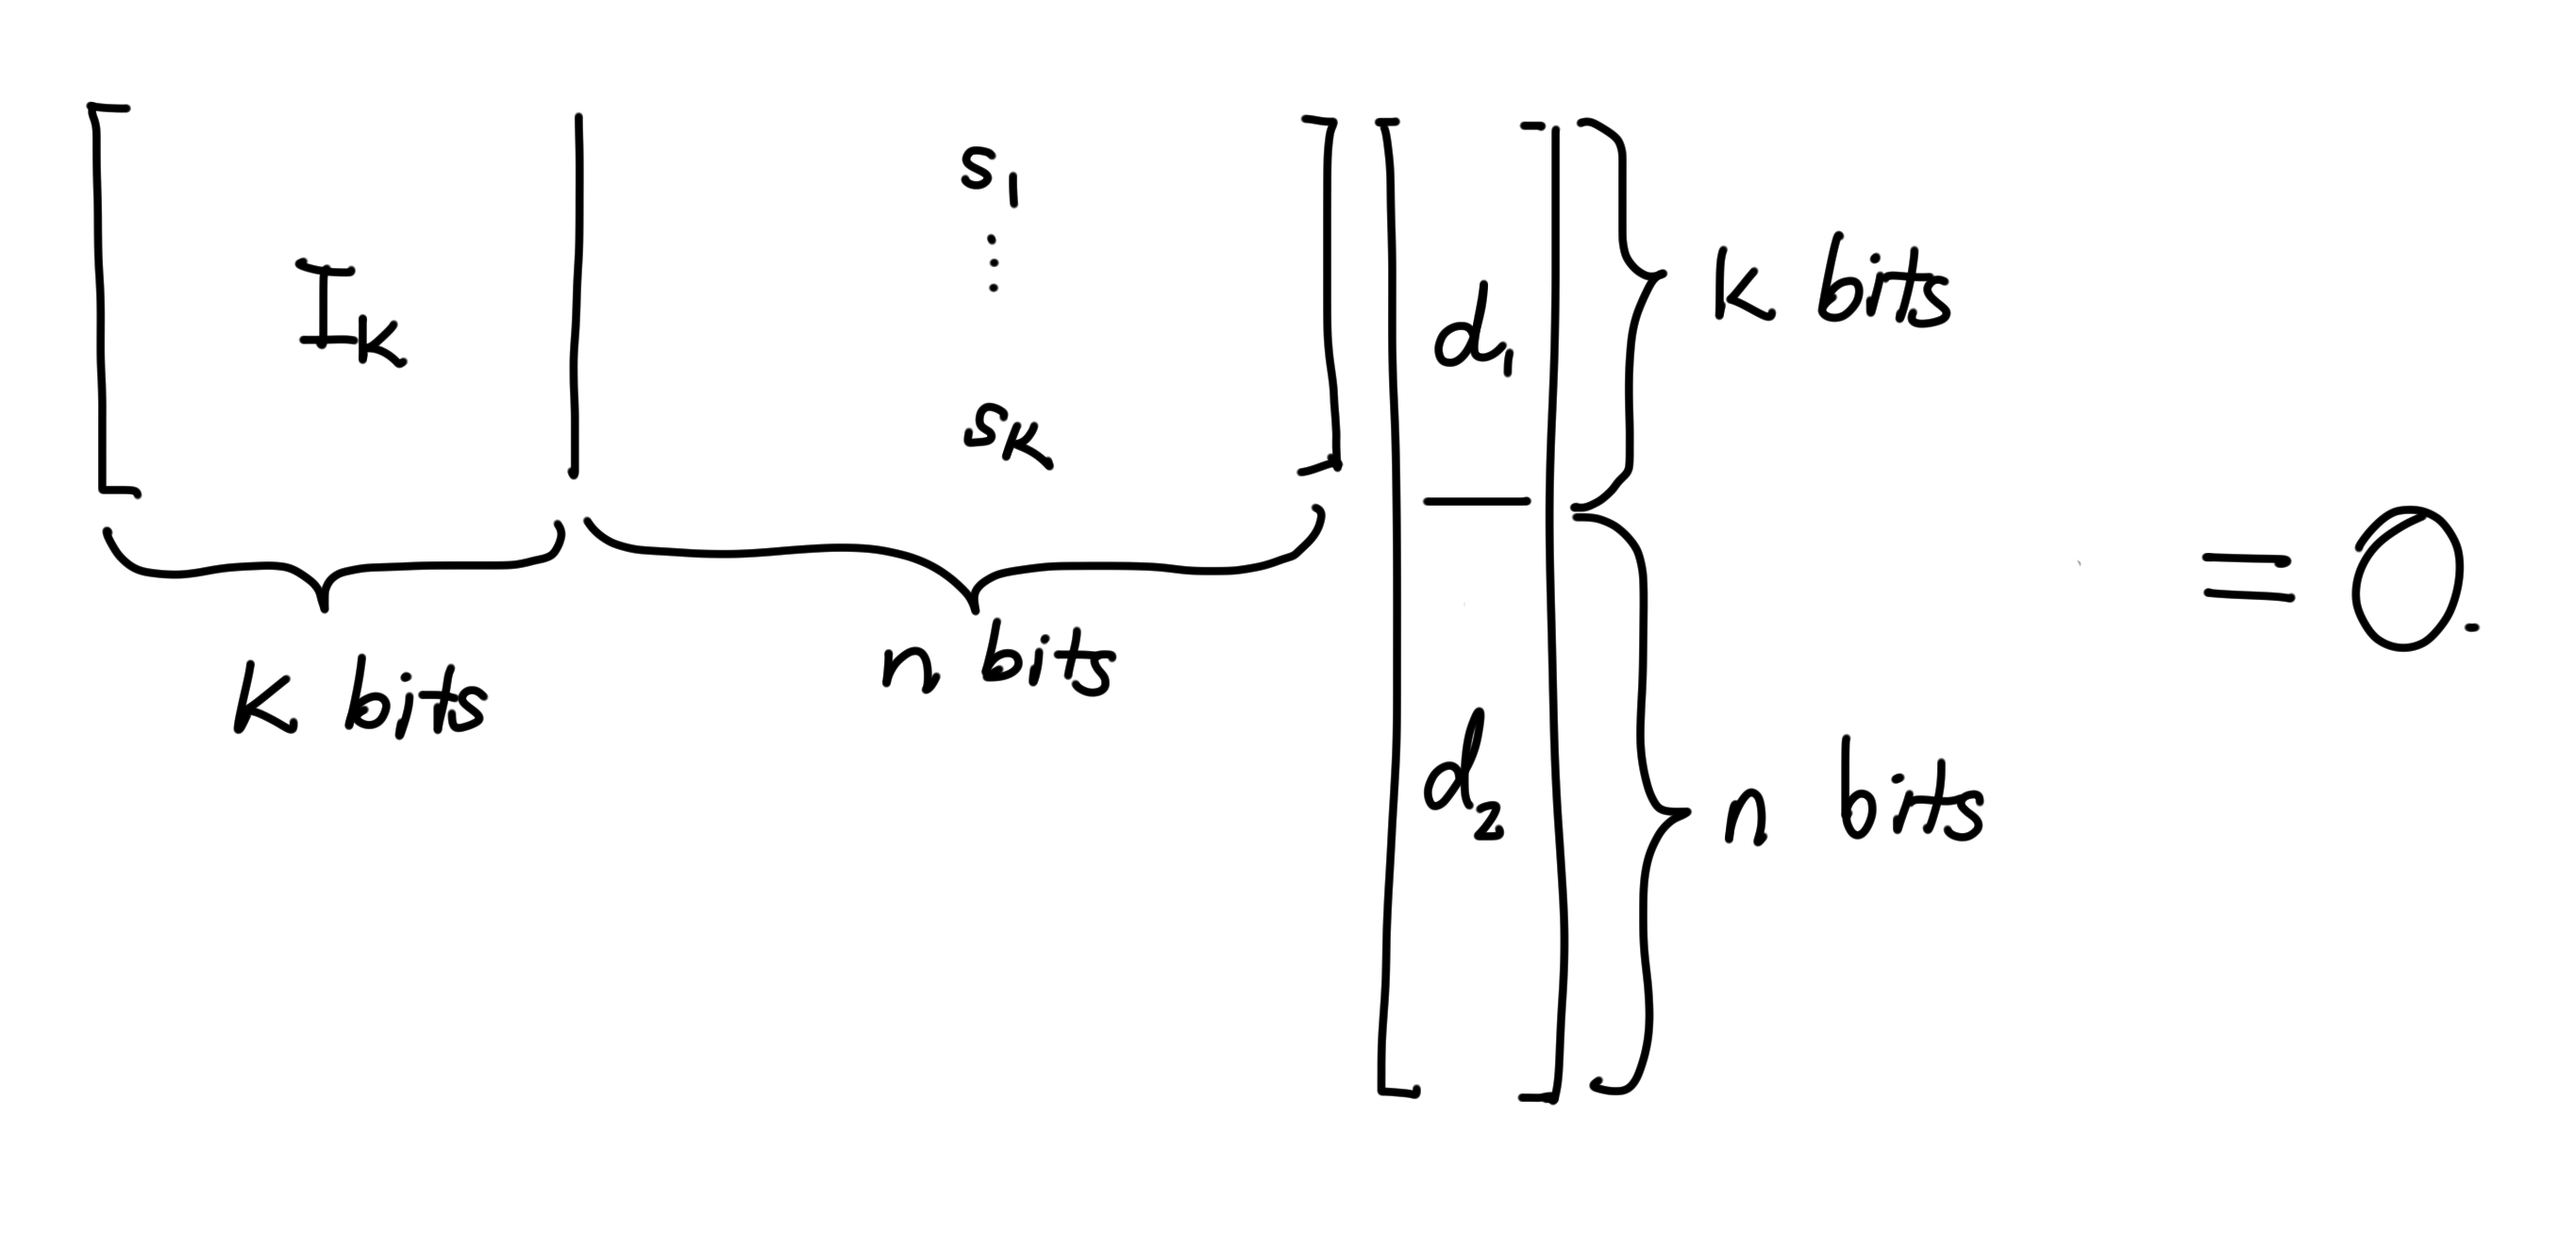
\includegraphics[width=0.8\textwidth]{Diagrams/1.png}
\end{center}

Note that this is equivalent to checking that, for all $i$, $d_2 \cdot s_i = d_{1, i}$ (where $d_{1, i}$ represents the $i$th bit of $d_1$).

We now prove that $F$ is non-collapsing, viz., there is an adversary $A$ (consisting of two phases, $A_0$ and $A_1$) who wins the collapsing game with non-negligible probability. When $A_0$ is called upon to provide a superposition over the message registers, it prepares the superposition

\begin{align}
	q^{-\frac{n}{2}} \sum_{\substack{b \in \{0,1\}^k \\ x \in \{0,1\}^n \\ e \in \mathbb{Z}_q^m}} \sqrt{D_{\mathbb{Z}_q^m, B_P}(e)} \ket{b, x, e}
\end{align}

(This superposition can be produced efficiently by creating the superposition $q^{-\frac{n}{2}} \sum_{e \in \mathbb{Z}_q^m} \sqrt{D_{\mathbb{Z}_q^m, B_P}(e)} \ket{e}$---which is possible by Lemma 3.12 of \cite{reg05}---and adding uniform superpositions over all $b$ and all $x$.)

The challenger evaluates $F$ on this superposition, and obtains the state
\begin{align}
    q^{-\frac{n}{2}} \sum_{\substack{b \in \{0,1\}^k \\ x \in \{0,1\}^n \\ e \in \mathbb{Z}_q^m}} \sqrt{D_{\mathbb{Z}_q^m, B_P}(e)} \ket{b, x, e} \Ket{A\big( L(x) \big) + e + A\big( L(s_b) \big) + e_b}.
\end{align}
The challenger then measures either the entire state or else the output register only, and returns one of the two following states to $A_1$:

\begin{itemize}
		\item $\ket{\psi_{\mathrm{meas}}} = \ket{b, x, e} \ket{F(b, x, e)}$ for some $(b, x, e)$.
     \item $\ket{\psi_y}$ for some $y$. We claim that $\ket{\psi_y}$ has (up to normalisation) the specific form 
		\begin{align}
			\ket{\psi_y} = \sum_b \sqrt{D_{\mathbb{Z}_q^m, B_P}(e^* - e_b)} \ket{b, x^* \oplus s_b, e^* - e_b} \ket{y}.
		\end{align}
		To show that it has this form, we prove the following lemma.
		
		\textbf{Lemma.} Fix a $y$. For each $b \in \{0,1\}^k$, there is exactly one $(x', e')$ with $x' \in \mathbb{F}_2^n, e' \in \mathbb{Z}_q^m$ such that $F(b, x', e') = y$, and it has the form $(x' = x^* \oplus s_b, e' = e^* - e_b)$, where $s_b = \bigoplus_i b_i s_i$, $e_b = \sum_i b_i e_i$, and ($x^*, e^*$) is the unique solution to the equation $A\big( L(x^*) \big) + e^* = y$.

		\textit{Proof.} Suppose that a $y$ has been measured. Note that this $y$ must be in the form $A\big( L(x^*) \big) + e^*$ for some $x^* \in \mathbb{F}_2^n$, and some $e^* \in \mathbb{Z}_q^m$ with sufficiently small magnitude. We recall that $L$ is injective, apply the inversion theorem (Theorem 5.1 of \cite{MP11}), and conclude that $(x^*, e^*)$ is unique. Given that this is so, the task of finding collisions becomes that of finding solutions $(b, x', e')$ to the following equation:
		\begin{align}
			A\big( L(x^*) \big) + e^* = A\big( L(x') \big) + e' + A\big( L(s_{b}) \big) + e_{b}.
		\end{align}
		The equation can be rearranged to yield:
		\begin{align}
			A\big( L(x') \big) + e' &= A\big( L(x^*) \big) + e^* - \Big( A\big( L(s_{b}) \big) + e_{b} \Big). \\
			\implies A\big( L(x') \big) + e' &= A\big( L(x^* \oplus s_{b}) \big) + e^* - e_{b}.
		\end{align}

		Applying the inversion theorem once again, we conclude that
		\begin{align}
			L(x') &= L(x^* \oplus s_{b}) \\
			\implies x' &= x^* \oplus s_{b}; \\
			e' &= e^* - e_{b}.
		\end{align}

		For each $b \in \{0,1\}^k$, there will be exactly one $(x', e')$ such that the pair of equations above are satisfied, and $x'$ and $e'$ have the form we claimed they would have. The lemma is thus proved.

		Given the lemma, it is clear that (up to normalisation)
		\begin{align}
			\ket{\psi_y} = \sum_b \sqrt{D_{\mathbb{Z}_q^m, B_P}(e^* - e_b)} \ket{b, x^* \oplus s_b, e^* - e_b} \ket{y}.
		\end{align}

		Since the maximum amplitude of $e_b$ is small compared to the Gaussian parameter of the distribution $D$, $\sqrt{D_{\mathbb{Z}_q^m, B_P}(e^* - e_b)}$ should be approximately the same for all $b$. In the following analysis, therefore, we replace the amplitudes in the above expression with a global normalisation factor. In other words,
		\begin{align}
			\ket{\psi_y} \approx \alpha \sum_b \ket{b, x^* \oplus s_b, e^* - e_b} \ket{y}.
		\end{align}
\end{itemize}

In order to tell whether it has been given $\ket{\psi_{\mathrm{meas}}}$ or $\ket{\psi_y}$, $A_1$ performs the following procedure.
\begin{itemize}
    \item Uncompute the $e$ register. This is possible because, using the hash function key, the value of the $e$ register for any member of the superposition can be computed from its corresponding values of $y$, $x$ and $b$.
    \item Apply the Hadamard transform to the remaining registers. In the case where $A_1$ was given $\ket{\psi_y}$, this results (up to normalisation) in the following state:
    \begin{align}
        \sum_d \bigg( \sum_b (-1)^{d \cdot (b \: || \: x^* \oplus s_b)} \bigg) \ket{d} = \sum_d \bigg( \sum_b (-1)^{d_1 \cdot b} (-1)^{d_2 \cdot (x^* \oplus s_{b})} \bigg) \ket{d}
    \end{align}
    Not all $d \in \{0,1\}^{n + k}$ will be supported in this superposition (and we will make precise which ones are). In the case where $A_1$ was given $\ket{\psi_{\mathrm{meas}}}$, however, every $d$ will appear in the superposition, because there will be no opportunity for the amplitude of $d$ to cancel.
    
    Note that, in the $\ket{\psi_y}$ case, we can rewrite the amplitude of $d$ in the following way:
    \begin{align}
        \sum_b (-1)^{d \cdot (b \: || \: x^* \oplus s_b)} &=
			\sum_b (-1)^{d_1 \cdot b} (-1)^{d_2 \cdot (x^* \oplus s_{b})} \\
        &= (-1)^{d_2 \cdot x^*} \sum_b (-1)^{d_1 \cdot b} (-1)^{d_2 \cdot \big( (x^* \oplus s_b) \oplus x^* \big)} \\
			&= (-1)^{d_2 \cdot x^*} \sum_b (-1)^{d_1 \cdot b} (-1)^{d_2 \cdot s_b} \\
			&= (-1)^{d_2 \cdot x^*} \sum_b (-1)^{\sum_i b_i \cdot (d_{1, i} \oplus d_2 \cdot s_i)} \\
			&= (-1)^{d_2 \cdot x^*} \prod_{i = 1}^n \big( 1 + (-1)^{d_{1, i} \oplus d_{2, i} \cdot s_i} \big)
    \end{align}
(22) is \textit{nonzero} if and only if $d_2 \cdot s_i = d_{1, i}$ for all $i$. Therefore, the only $d$s that will be supported in the superposition after Hadamard are those such that $P(d) = 1$.

	\item Apply $P$ to the superposition of $d$s and measure the result. If $A_1$ was given $\ket{\psi_y}$, this measurement will yield 1 with probability 1. If $A_0$ was given $\ket{\psi_{\mathrm{meas}}}$, the probability that this measurement yields 1 is negligible, because the probability $Pr\Big[ d \in S_0 \: \Big| \: d \stackrel{r}{\leftarrow} \mathbb{F}_2^{n+k} \Big]$ is exponentially small if $k$ is linear in $n$. This completes the proof that $A$ wins the collapsing game with non-negligible probability $1 - \textsf{negl}(n)$.
\end{itemize}

\subsection{Collision resistance}
Note that, if an adversary can recover $\big( (b, x, e), (b', x', e') \big)$ such that $F(b, x, e) = F(b', x', e')$, he can evaluate $x \oplus x'$ and recover $s_{\hat b}$ for some $\hat b$. Therefore, in order to prove that it is impossible to find collisions, we prove that it is impossible to recover any $s_{\hat b} = \bigoplus_i \hat b_is_i$ given the hash function key. We do so through a sequence of hybrids.

\begin{itemize}
    \item $H_0$: The challenger outputs the key as it is defined in section 4.1.
    \item $H_1$: Relying upon the security of \textsf{shO}, the challenger swaps $P$ for another subspace membership program that instead checks membership in a random, higher-dimensional subspace $S_1 \supset S_0$. $H_0$ and $H_1$ are indistinguishable by the security of \textsf{shO}.
    \item $H_2$: The challenger gives out a full description of $S_1$, instead of a membership program. Any adversary who can break collision resistance in $H_1$ can also do so in $H_2$.
    \item $H_3$: The challenger outputs $k$ random strings instead of the samples $A\big( L(s_i) \big) + e_i$. It also outputs $S_1$ and $A$ as before.

We show that this hybrid and the last are indistinguishable by reducing the problem of telling them apart to the problem of decisional LWE with secrets drawn from any distribution $\mathcal{D}$ that has sufficient entropy (\cite{robustness}). Following \cite{robustness}, we denote this problem by \textsf{DLWE}($\mathcal{D}$).

	  Let $C$ be the following probabilistic algorithm (which takes $S_1$ as argument):
    \begin{itemize}
        \item Choose a random $k \times (n+k)$ matrix $M$ whose kernel is in $S_1$. On average (for large $k$), at least 1 in every 4 of such randomly chosen $M$ will have the property that its first $k$ columns are linearly independent.\footnote{This is because the product $\prod_{i=1}^k \big(1-(\frac{1}{2})^{k+1-i}\big)$, which represents the probability that $k$ randomly chosen vectors in $\mathbb{F}_2^k$ will be linearly independent, is known to converge to a constant $ > \frac{1}{4}$ as $k \rightarrow \infty$.} Repeat the choosing procedure until an $M$ with this property is found.
        \item Row reduce $M$ until it is in the form $I_k \: | \: \mathcal{S}'$.
        \item Output $\mathcal{S}'$.
    \end{itemize}

By the $\textsf{DLWE}(\mathcal{D})$ assumption, where $\mathcal{D}$ is the uniform distribution over the set $\{L(\mathcal{S}'^T) \:|\: \mathcal{S}' \leftarrow C(S_1)\}$, no adversary can tell the difference between the samples $A\big( L(s_i) \big) + e_i$ and $k$ random strings. Suppose there were an adversary $A$ who could. We enlist $A$ to build an adversary $B$ who breaks $\textsf{DLWE}(\mathcal{D})$. $B$ receives a random LWE sample $\Big(A, A\big( L(\mathcal{S}'^T) \big) + E \Big)$, where $A$ is an $m \times n$ matrix, $L(\mathcal{S}'^T)$ is an $n \times k$ matrix, and $E$ is an $m \times k$ matrix; $B$ also knows the distribution $\mathcal{D}$, which means that it knows $S_1$ and can provide $A$ with a description of it. Notice that the columns of $B$'s sample constitute $k$ vectors of the form $A\big( L(s_i) \big) + e_i$. Therefore, $B$ gives its sample to $A$ column-wise, and outputs whatever $A$ outputs. If $A$ can distinguish between $H_3$ and $H_2$, then $B$ can break $\textsf{DLWE}(\mathcal{D})$. We conclude that $H_3$ and $H_2$ are indistinguishable.
	\item $H_4$: The challenger simply outputs $S_1$. It is clearly impossible to recover $\mathrm{span}(s_1, \cdots, s_k)$---or any member of that subspace---with non-negligible probability from only $S_1$, provided that the dimension gap $d_1 - d_0$ (where $d_1$ is the dimension of $S_1$, and $d_0$ is the dimension of $S_0$) is linear in $n$: there are exponentially many equally probable possibilities, and the adversary has no way of distinguishing between them. This completes our proof that $F$ is collision resistant.
\end{itemize}

\bibliographystyle{alpha}
\bibliography{bibliography}
\end{document}
